Ein kugelförmiger Wassertropfen vom Radius 1 bricht parallel einfallende
Lichtstrahlen.
In Aufgabe~\ref{10000099} wurde gezeigt, dass der an der ersten Kugelfläche
gebrochene Strahl vier Einheiten hinter der Fläche die Achse kreuzt.
Durch die zweite Kugelfläche wird diese Distanz nochmals verkürzt.
Der Brechungsindex von Wasser ist $n=\frac43$.
Wo befindet sich der Brennpunkt?

\begin{center}
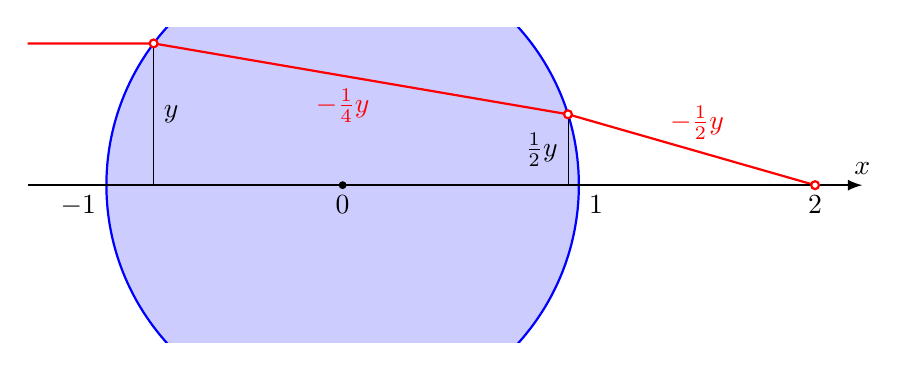
\begin{tikzpicture}[>=latex,thick]
\def\R{3}
\def\y{1.8}
\clip (-4,-2) rectangle (7,2);
\fill[color=blue!20] (0,0) circle[radius=\R];
\draw[color=blue] (0,0) circle[radius=\R];
\draw[line width=0.3pt] ({-sqrt(\R*\R-\y*\y},0) -- ++(0,\y);
\node at ({-sqrt(\R*\R-\y*\y},{0.5*\y}) [right] {$y$};
\draw[line width=0.3pt] ({sqrt(\R*\R-0.25*\y*\y},0) -- ++(0,{0.5*\y});
\node at ({sqrt(\R*\R-0.25*\y*\y},{0.25*\y}) [left] {$\frac12y$};
\draw[color=red] (-4,\y)
	-- ({-sqrt(\R*\R-\y*\y)},\y)
	-- ({sqrt(\R*\R-0.25*\y*\y)},{0.5*\y})
	-- ({\R*2},0);
\node[color=red] at ({1.5*\R},{0.25*\y}) [above] {$-\frac12 y$};
\node[color=red] at (0,{0.75*\y}) [below] {$-\frac14 y$};
\draw[->] (-4,0) -- (6.6,0) coordinate[label={$x$}];
\fill[color=white] ({-sqrt(\R*\R-\y*\y)},\y) circle[radius=0.05];
\draw[color=red] ({-sqrt(\R*\R-\y*\y)},\y) circle[radius=0.05];
\fill[color=white] ({sqrt(\R*\R-0.25*\y*\y)},{0.5*\y}) circle[radius=0.05];
\draw[color=red] ({sqrt(\R*\R-0.25*\y*\y)},{0.5*\y}) circle[radius=0.05];
\fill[color=white] ({\R*2},0) circle[radius=0.05];
\draw[color=red] ({\R*2},0) circle[radius=0.05];
\fill (0,0) circle[radius=0.05];
\node at (0,0) [below] {$0$};
\node at (-\R,0) [below left] {$-1$};
\node at (\R,0) [below right] {$1$};
\node at ({\R*2},0) [below] {$2$};
\end{tikzpicture}
\end{center}

\begin{loesung}
Die beiden Brechungsmatrizen sind
\begin{align}
B(1,n,1)
&=
\begin{pmatrix}
1&0\\
-\frac14&\frac34
\end{pmatrix}
\\
B(n,1,1)
&=
\begin{pmatrix}
1&0\\
-(\frac43-1)&\frac43
\end{pmatrix}
=
\begin{pmatrix}
1&0\\
-\frac13&\frac43
\end{pmatrix}
\end{align}
Der Abstand zwischen den beiden Flächen ist 2, dargestellt durch die Matrix
\[
T_2 =
\begin{pmatrix}
1&2\\
0&1
\end{pmatrix}.
\]
Das ganze System wird daher durch das Produkt
\[
T
=
B(n,1,1)T_2B(1,n,1)
=
\begin{pmatrix}
1&0\\
-\frac13&\frac43
\end{pmatrix}
\begin{pmatrix}
1&2\\
0&1
\end{pmatrix}
\begin{pmatrix}
1&0\\
-\frac14&\frac34
\end{pmatrix}
=
\begin{pmatrix}
1&2\\
-\frac13&\frac23
\end{pmatrix}
\begin{pmatrix}
1&0\\
-\frac14&\frac34
\end{pmatrix}
=
\begin{pmatrix}
\frac12 & \frac32 \\
-\frac12 & \frac12
\end{pmatrix}.
\]
Der im Abstand $y$ von der Achse ankommende Strahl wird auf
\[
\begin{pmatrix}
\frac12 & \frac32 \\
-\frac12 & \frac12
\end{pmatrix}
\begin{pmatrix}y\\0\end{pmatrix}
=
\begin{pmatrix}\frac12y\\-\frac12y\end{pmatrix}
\]
gebrochen.
Der Strahl verlässt also die Wasserkugel im Abstand $\frac12y$ von der
Achse mit Steigung $-\frac12y$, er schneidet daher die $x$-Achse
$\frac12y/\frac12y=1$ Einheiten weiter hinten.
\end{loesung}
